\subsection{Layer 3 (Network)}
\subsection*{Aufgaben}
\begin{itemize}
	\item Routing
	\item Globale Adressierung
	\item Kommunikation mit L2 \& L4
\end{itemize}
\textbf{Protkolle:} IPv4, IPv6, ICMP, RIP, OSPF, EIGRP, IS-IS, BGP

\subsection*{IPv4}
Eigenschaften von IP
\begin{itemize}
	\item Verbindungslos
	\item Best Effort
	\item Medium unabhängig
\end{itemize}
\textbf{IP-Header (8.2.2)}
Wichtige Felder: Source \& Destination IP, Time-to-Live

\subsection*{Kommunikationsart}
\begin{itemize}
	\item Unicast (IP des Host)
	\item Multicast (224.0.0.0 - 239.255.255.255)
	\item Broadcast (letzte IP im Netz, 255.255.255.255)
\end{itemize}

\subsection*{Spezielle IP-Adressen}
\begin{itemize}
	\item 127.0.0.0 / 8 ... localhost
	\item 10.0.0.0 / 8
	\item[] 172.16.0.0 / 12
	\item[] 192.168.0.0 / 16 ... private IP-Adressen (NAT)
	\item 169.254.0.0 / 16 ... APIPA
	\item 192.0.2.0 / 24 ... Testnetz
\end{itemize}
\textbf{Fazit:} Zu wenig IPv4-Adressen!

\subsection*{Deshalb}
\begin{itemize}
	\item VLSM (variable length subnet mask)
	\item NAT
	\item IPv6
\end{itemize} 

\subsection*{Classful Addressing (uralt)}
Das erste Oktett bestimmt die Subnetzmaske (/8, /16, /24)
\begin{table}[H]
	\begin{tabular}{ccll}
		Klasse A & 0-127 & (0...) & /8 \\
		Klasse B & 128-191 & (10...) & /16 \\
		Klasse C & 192-223 & (110...) & /24 \\
		Klasse D & 224-239 & (1110...) & Multicast \\
		Klasse E & 240-255 & (11110...) & für spätere Verwendung
	\end{tabular}
\end{table}

\subsection*{Classless Addressing (veraltet!)}
Die Subnetzmasken /8, /16, /24 können beliebig verwendet werden

\subsection*{CIDR (Classless Inter-Domain Routing)}
Es können beliebige Subnetzmasken (z.B. /25, /26, ...) verwendet werden. Alle Subnetze werden gleich groß.

\subsection*{VLSM (variable length subnet mask)}
Alle Subnetzmasken können beliebig verwendet werden. Die Netzte dürfen sich nicht überschneiden.

\subsection*{Subnetzmasken}
\begin{table}[H]
	\begin{tabular}{cccl}
		Präfix Notation & Dotted Decimal Notation & Hosts & Subnetz von /24 \\
		/25 & 255.255.255.128 & $2^{7}$ - 2 = 126 & 2 \\
		/26 & 255.255.255.192 & $2^{6}$ - 2 = 62 & 4 \\
		/27 & 255.255.255.224 & $2^{5}$ - 2 = 30 & 8 \\
		/28 & 255.255.255.240 & $2^{4}$ - 2 = 14 & 16 \\
		/29 & 255.255.255.248 & $2^{3}$ - 2 = 6 & 32 \\
		/30 & 255.255.255.252 & $2^{2}$ - 2 = 2 & 64 \\
		/31 & 255.255.255.254 & $2^{1}$ - 2 = 0 & für spezielle Anwendung \\
		/20 & 255.255.240.0 & $2^{12}$ - 2 = 4.094 & /
	\end{tabular}
\end{table}

\subsection*{Bsp 1 (CIDR):}
\begin{figure}[H]
	\centering
	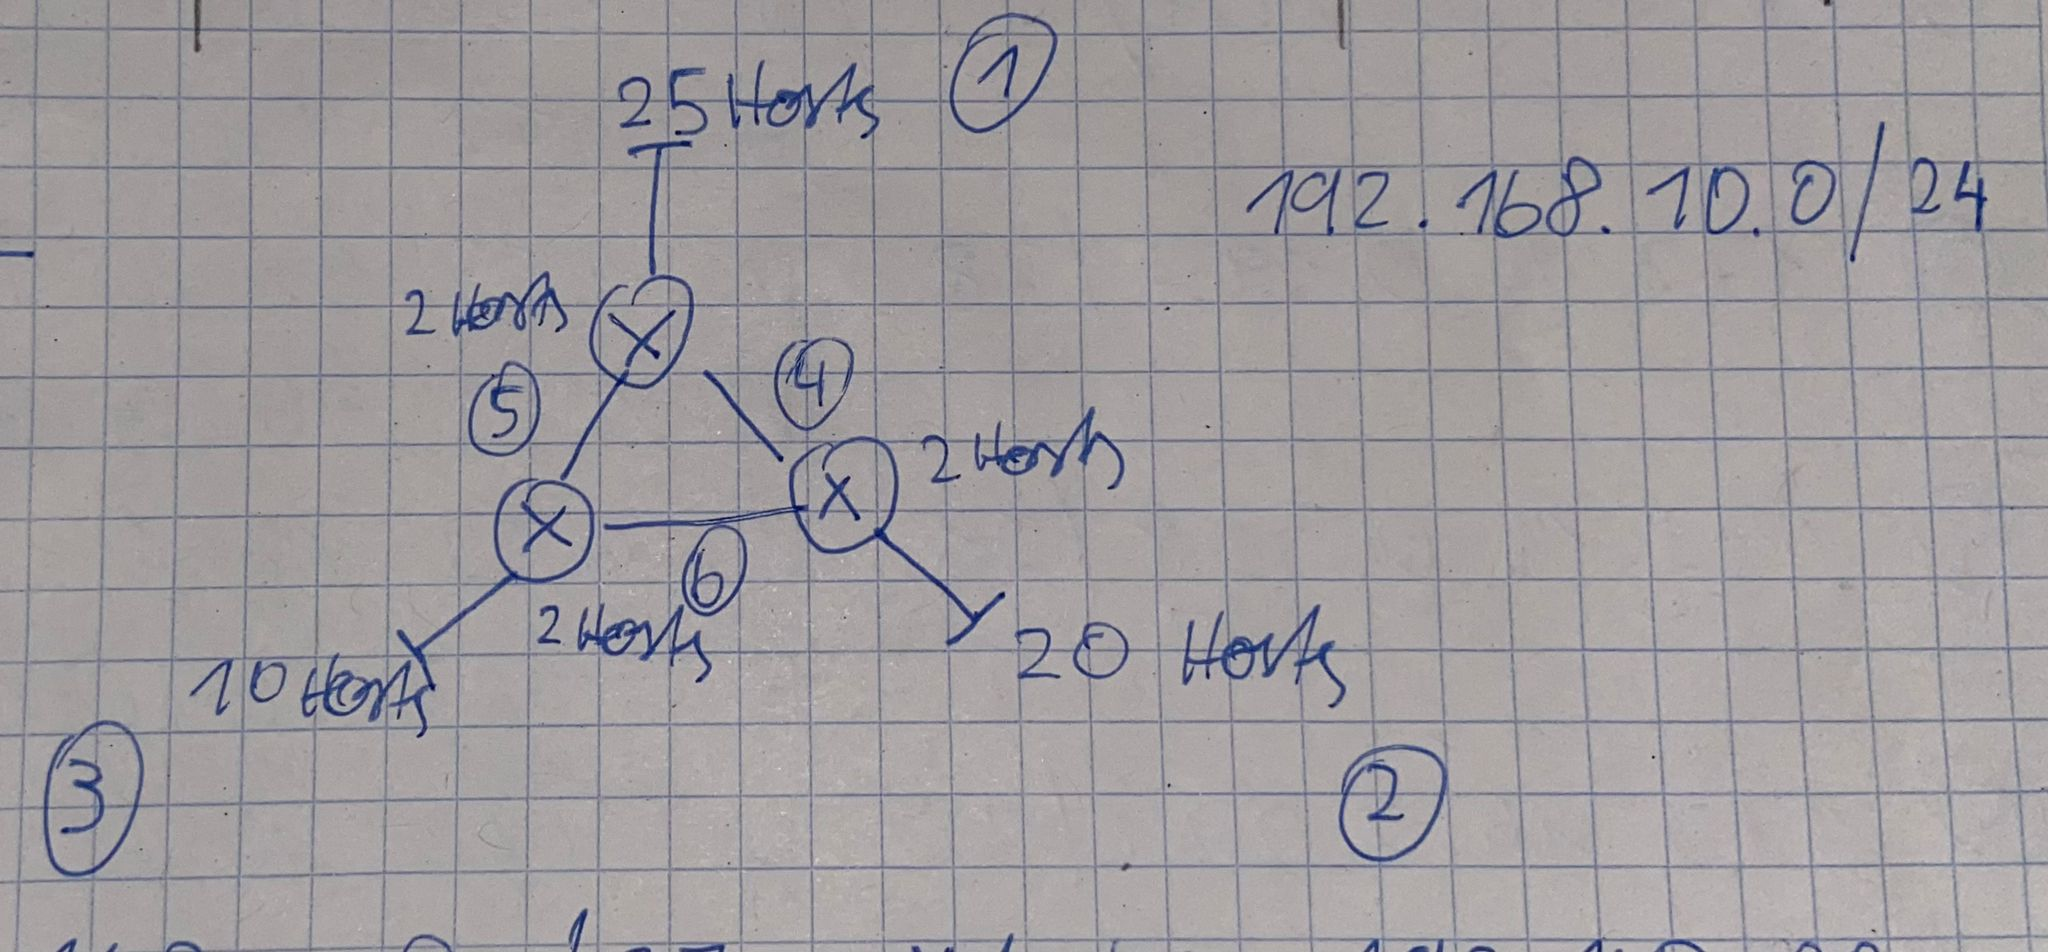
\includegraphics[width=1.0\linewidth]{figures/bsp1_cidr.jpeg}
	\caption{CIDR Beispiel}
\end{figure}
\begin{table}[H]
	\begin{tabular}{llll}
		1 & 192.168.10.0 / 27 & Netzadresse & 192.168.100.0 \\
		&  & Broadcast & 192.168.100.31 \\
		\hline
		2 & 192.168.10.32 / 27 & Netzadresse & 192.168.100.32 \\
		&  & Broadcast & 192.168.100.63 \\
		\hline
		3 & 192.168.10.64 / 27 & Netzadresse & 192.168.100.64 \\
		&  & Broadcast & 192.168.100.95 \\
		\hline
		4 & 192.168.10.96 / 27 & Netzadresse & 192.168.100.96 \\
		&  & Broadcast & 192.168.100.127 \\
		\hline
		5 & 192.168.10.128 / 27 & Netzadresse & 192.168.100.128 \\
		&  & Broadcast & 192.168.100.159 \\
		\hline
		6 & 192.168.10.160 / 27 & Netzadresse & 192.168.100.160 \\
		&  & Broadcast & 192.168.100.191
	\end{tabular}
\end{table}

\subsection*{Bsp 2 (VLSM):}
\begin{figure}[H]
	\centering
	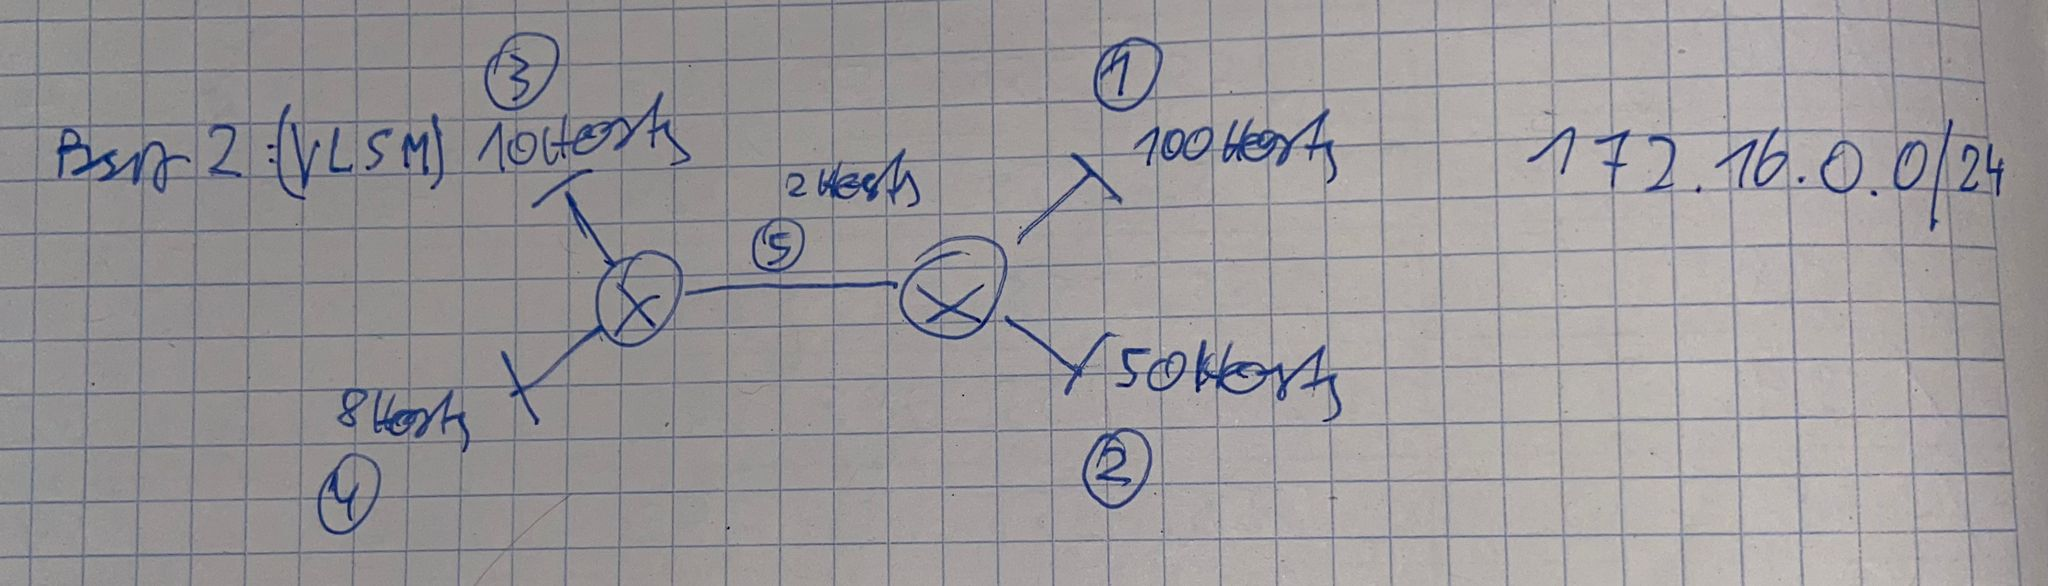
\includegraphics[width=1.0\linewidth]{figures/bsp2_vlsm.jpeg}
	\caption{VLSM Beispiel}
\end{figure}
\begin{table}[H]
	\begin{tabular}{llll}
		1 & 172.16.0.0 / 25 & Netzadresse & 172.16.0.0 \\
		&  & Broadcast & 172.16.0.127 \\
		\hline
		2 & 172.16.0.128 / 26 & Netzadresse & 172.16.0.128 \\
		&  & Broadcast & 172.16.0.191 \\
		\hline
		3 & 172.16.0.192 / 28 & Netzadresse & 172.16.0.192 \\
		&  & Broadcast & 172.16.0.207 \\
		\hline
		4 & 172.16.0.208 / 28 & Netzadresse & 172.16.0.208 \\
		&  & Broadcast & 172.16.0.223 \\
		\hline
		5 & 172.16.0.224 / 30 & Netzadresse & 172.16.0.224 \\
		&  & Broadcast & 172.16.0.227
	\end{tabular}
\end{table}

(PT: 10.4.3, 11.5.5, 11.9.3, 11.10.1)






